\documentclass[oneside,12pt,enabledeprecatedfontcommands]{scrreprt}
\usepackage{graphicx}
\usepackage[ngerman]{babel} %Deutsche Sprachunterstützung
\usepackage{scrpage2} %Kopf- und Fußzeilen
\usepackage[utf8]{inputenc} %Umlaute
\usepackage{eso-pic} % background
\usepackage{soul} %Striketrough \st{}

\newcommand\AtPageUpperRight[1]{\AtPageUpperLeft{%
 \put(\LenToUnit{\paperwidth},\LenToUnit{0\paperheight}){#1}%
 }}%
 
 \newcommand\BackgroundPic{%
\put(0,0){%
\parbox[b][\paperheight]{\paperwidth}{%
\vfill
\centering
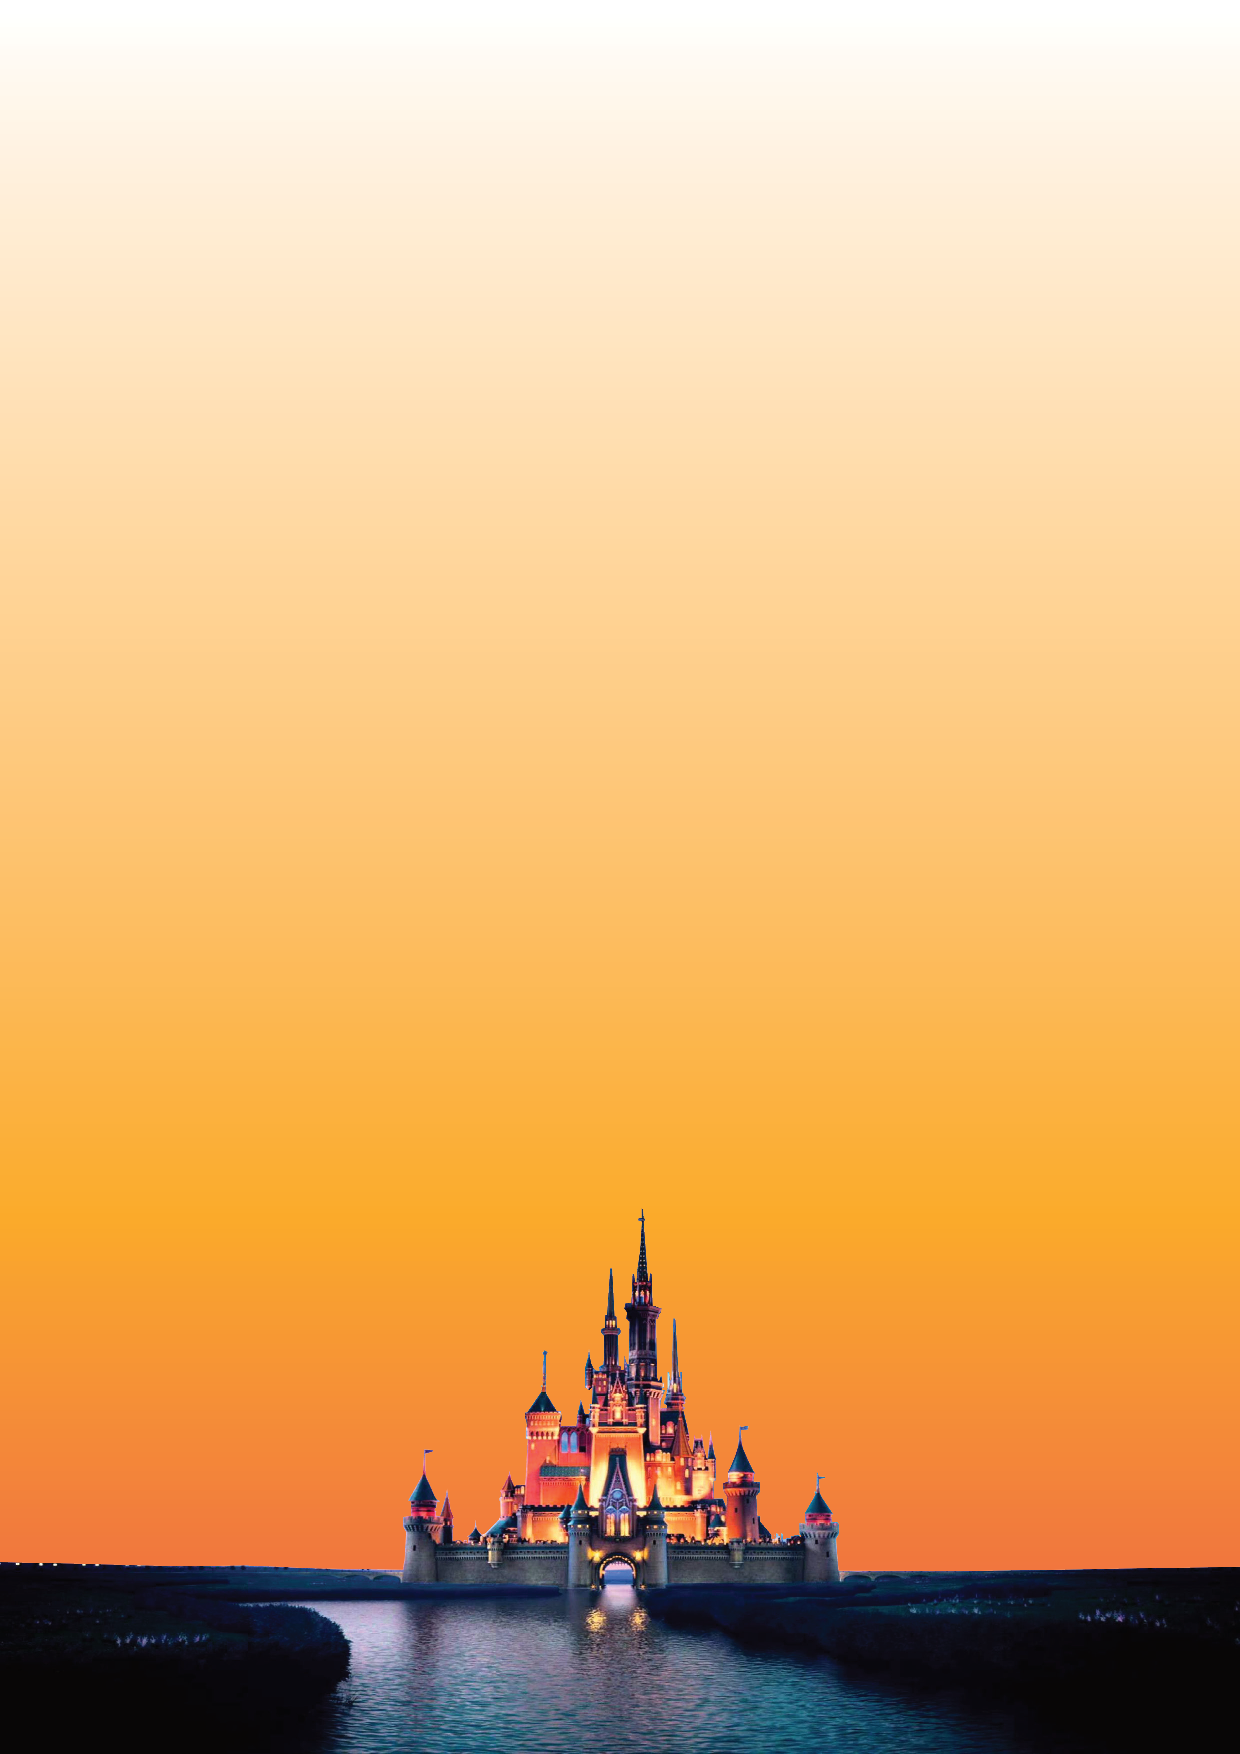
\includegraphics[width=\paperwidth,height=\paperheight,%
keepaspectratio]{../../res/Background/Disney_Background}%
\vfill
}}}

\begin{document}
\AddToShipoutPicture*{\BackgroundPic}
\AddToShipoutPictureBG*{%
  \AtPageUpperLeft{\raisebox{-\height}{
\includegraphics[scale=.15,trim=50mm 0mm 100mm -10mm]{../../res/TEN_SING_Logo}}}%
  \AtPageUpperRight{\put(-100,-6){\raisebox{-\height}{
\includegraphics[scale=.18,trim=50mm 0mm 100mm -10mm]{../../res/CVJM_Logo_Vektor_Rein}}}}%
}
\begin{center}
\phantom{asdf}
\vspace{-2.5cm}
+++ Version 2 vom 15. März 2017 +++


\includegraphics[scale=.3]{../../res/Walt_Disney_Pictures_Castle_Logo-Crop}

\vspace{-1cm}
\Huge{Drama präsentiert}:

\vspace{2cm}
%\lipsum[1]
\Huge\textbf{Unser super-mega-krass-tolles Disney-Theaterstück!!1!}\\
\textit{(wir haben noch kein Motto)}

\vspace{1cm}

\Large \st{+++ ihre Werbung hier +++ ihre Werbung hier +++}

\vspace{1.5cm}

\Large TenSing Moers, 2017
\end{center}
\end{document}